\documentclass[upright, contnum]{umemoria}
\depto{DEPARTAMENTO DE CIENCIAS DE LA COMPUTACI�N}
\author{WILLY ADOLFO MAIKOWSKI CORREA}
\title{REDISE�O E IMPLEMENTACI�N DE UN SISTEMA DE RECUENTO DE UNIDADES DOCENTES PARA LA FACULTAD DE CIENCIAS F�SICAS Y MATEM�TICAS}
\auspicio{}
\date{OCTUBRE 2015}
\guia{PATRICIO POBLETE OLIVARES}
\carrera{INGENIERO CIVIL EN COMPUTACI�N}
\memoria{MEMORIA PARA OPTAR AL T�TULO DE}
\comision{JAVIER VILLANUEVA GONZ�LEZ}{\ }{\ }

\usepackage{lipsum}

\usepackage[latin1]{inputenc}
\usepackage[T1]{fontenc}

\begin{document}

\frontmatter
\maketitle

\begin{abstract}
{\lipsum[1-4]}
\end{abstract}

\begin{dedicatoria} % opcional
Una dedicatoria corta. Por ejemplo, \emph{A los creadores de U-Campus}
\end{dedicatoria}

\begin{thanks} % opcional
\lipsum[1-2]
\end{thanks}
\cleardoublepage

\tableofcontents
\listoftables % opcional
\listoffigures % opcional

\mainmatter

\begin{intro}

	Hace alg�n tiempo en la Facultad de Ciencias Fisicas y Matematicas de la Universidad de Chile, en una etapa previa del proceso de titulaci�n se deb�a realizar un recuento manual de 
	los ramos y sus respectivos cr�ditos (Unidades Docentes o UDs). Esto quiere decir que se deb�a corroborar los ramos aprobados con el respectivo plan y t�tulo que se quer�a obtener. 
	Este trabajo que parec�a sencillo, result� ser arduo y complejo, lo que implicaba que una solicitud de recuento demorara meses en ser calculada.

	A partir del a�o 2013 el �rea de Infotecnolog�as (ADI) implement� un sistema de recuentos autom�tico para apoyar esta labor manual, el que implic� una mejora considerable, 
	permitiendo que la misma labor pasara de realizarse de meses a segundos.

	El problema consiste en verificar si un alumno espec�fico cumple con un plan de estudios. Cuando hay m�s de una manera posible de que el plan se cumpla, se busca maximizar la nota 
	con la que deber�a egresar. La tarea de comprobar el cumplimiento del plan actualmente no est� siendo abarcada en su totalidad. El sistema puede calcular que un alumno no cumple 
	con un plan cuando realmente s� lo hace (falso negativo). Lo anterior se considera cr�tico. 

	Tambi�n hay problemas respecto del promedio de titulaci�n que entrega el sistema. Como es posible que un plan de estudios se cumpla a trav�s de distintas combinaciones de cursos y 
	a la forma en que est� implementada la soluci�n, se alcanzan a examinar s�lo algunos resultados posibles, pero no necesariamente se encuentra el �ptimo global. 

	Aunque institucionalmente no es parte del reglamento el que se deba maximizar la nota del avance curricular, esto es de gran inter�s para el alumnado, por lo que es parte de lo que 
	se pretende mejorar.

	Las preocupaciones descritas anteriormente provocan que este recurso, si bien es ampliamente ocupado, se utilice s�lo como informaci�n referencial, debi�ndose revisar posibles 
	errores. Todo lo antes descrito motiv� la propuesta de este tema para mejorar el actual sistema. 

	%\begin{enumerate}
	%	\item Item 1
	%		\begin{enumerate}
	%			\item Subitem 1
	%			\item Subitem 2 (ver Figura \ref{logofcfm})
	%		\end{enumerate}
	%	\item Item 2
	%	\item Item 3
	%\end{enumerate}
	%\begin{teo}
	%	Se tiene que $$\int_0^t e^sds=e^t-1.$$
	%\end{teo}
	%\lipsum[36-40]
\end{intro}

\chapter{Primero}
\lipsum[1-3]
\begin{defn}[ver \cite{KAR00}] Definici�n definitiva $$\frac{d}{dx}\int_a^xf(y)dy=f(x).$$\end{defn}
\chapter{Marco Te�rico}

Gran parte de los conceptos utilizados en esta memoria no son necesariamente de conocimiento general. Es por ello que a continuaci�n se explicara de manera breve los elementos m�s utilizados.

\section{Complejidad}

Cuando se desean comparar procedimientos o algoritmos se debe utilizar alguna unidad de medida que permita definir cual es mejor. Una unidad importante es el tiempo (cuanto tiempo demora uno con respecto al otro) pero este es relativo a la cantidad de datos que se procesan, por ejemplo, es distinto intentar ordenar cien n�meros a ordenar un mill�n. Por lo anterior, para comparar dos procedimientos, com�nmente se define una funci�n $T(n)$ donde $n$ es la variable que define el tama�o de los datos.

A partir de estos hechos y del procesamiento de los datos que se realiza en el algoritmo, se va describiendo el comportamiento de la funci�n. Por ejemplo, si el algoritmo visita dos veces cada uno de los datos la funci�n estar�a definida por $T(n) = 2 \cdot n$. 

Hay que tener en consideraci�n, adem�s, que esta definici�n es independiente de la tecnolog�a utilizada para procesar. Es decir, si utilizamos una maquina con mayor capacidad se procesar� una cantidad de datos determinada mucho mas r�pido pero seguir� teniendo la misma funci�n, por lo tanto es com�n enunciar la tecnolog�a utilizada.

Usualmente no es utilizada directamente la funci�n $T(n)$ y se usan asintotas que determinan el mejor y peor caso en que se puede comportar el algoritmo. Esto permite un an�lisis mas r�pido debido a reducciones que se pueden utilizar. En esta memoria se trabajar� con el peor caso que se denota con una letra $O$. Debido a la descripci�n de esta ultima funci�n se puede tener distintos tipos de complejidades, por ejemplo cuando se tiene una funci�n $O(n^2)$ se dice que esta tiene un comportamiento cuadr�tico para hacer referencia al polinomio de segundo grado o cuando se tiene una funci�n $O(3^n)$ se dice que es de orden exponencial debido a que la variable se encuentra en el exponente.

\begin{figure}[!h]
	\centering
	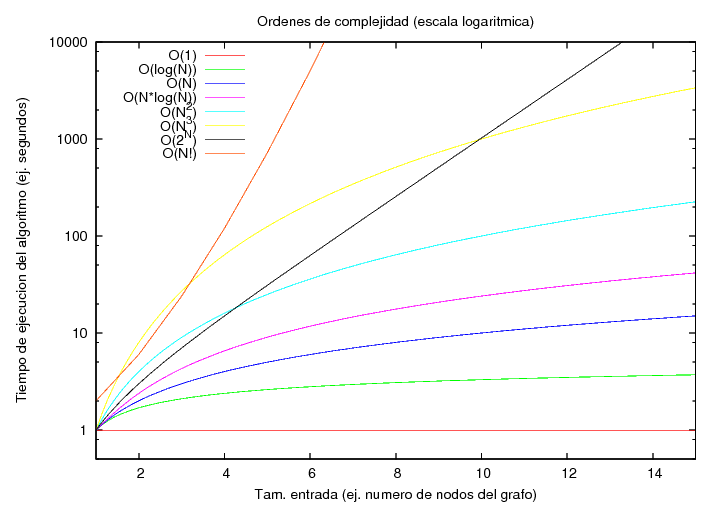
\includegraphics[scale=0.6]{imagenes/5}
	\caption{Grafico con las curvas de los ordenes de complejidad en una escala logaritmica}
	\label{ordenes}
\end{figure}

En la figura \ref{ordenes} se pueden ver los tiempos que demora en procesar un algoritmo una cantidad de datos determinada en una escala logar�tmica donde mientras m�s arriba diverge la funci�n m�s dif�cil o m�s tiempo toma su calculo. En computaci�n se tienen distintos tipos de clases de complejidad para clasificar los problemas seg�n la mejor soluci�n descubierta por el momento siendo las mas conocidas la clase P, los problemas que pueden ser resueltos en tiempo polinomial, y NP, los problemas que pueden ser resueltos en tiempo polinomial pero solo por una maquina no determinista. Estos �ltimos poseen un subconjunto de problemas conocidos con una complejidad mucho mayor y que son reducibles entre ellos, es decir, un problema puede ser representado o transformado a una variante equivalente de otro problema dentro de ese subconjunto.

Otra unidad de medida diferente al tiempo es la unidad de espacio. Con esto se eval�a la cantidad de memoria necesaria que requiere una soluci�n. En esta tesis se tendr� �nfasis en la unidad de tiempo pero en la secci�n ``Validaci�n'' se mencionar� brevemente los cuidados que hay que tener con el espacio.


\section{Teor�a de Grafos}

Un campo que ha tomado gran importancia en la computaci�n es la teor�a de grafos. Los grafos son una estructura que esta compuesta por dos elementos: los nodos y las aristas. Las aristas pueden tener direcci�n y en ese caso se habla de un grafo dirigido.

\begin{figure}[!h]
	\centering
	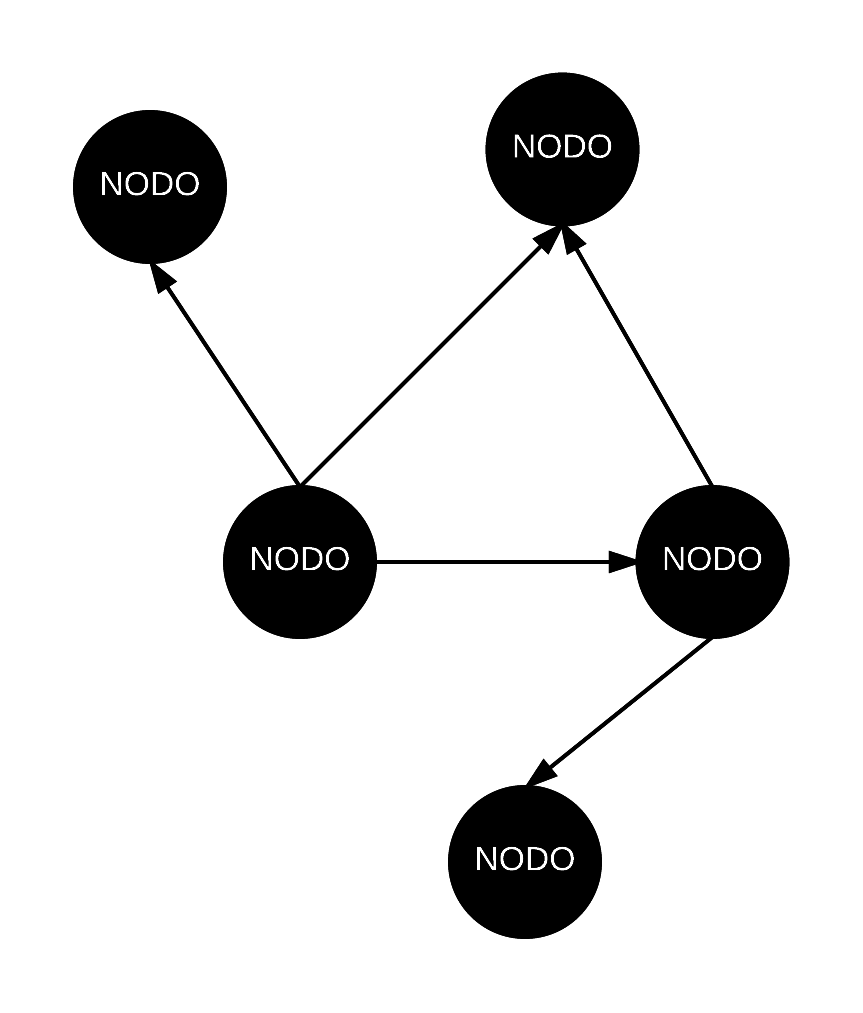
\includegraphics[scale=0.9]{imagenes/6}
	\caption{Ejemplo de grafo dirigido}
	\label{directed_graph}
\end{figure}

La forma que posee esta estructura ha sido de utilidad debido a que muchas cosas pueden representarse mediante ella. Por ejemplo, posiciones dentro de un mapa pueden ser representadas por nodos y las aristas son los caminos entre ellas teniendo la habilidad de agregar valores (la arista tiene un valor mayor mientras mas alejados est�n los nodos). A partir de esto y una representaci�n matem�tica de los elementos de un grafo pueden resolverse problemas te�ricos con variada utilidad en la practica. Siguiendo el mismo ejemplo anterior, la soluci�n te�rica del camino con aristas de menor valor entre dos nodos podr�a representar el camino mas corto entre dos lugares geogr�ficos.

Existen variados tipos de grafos entre ellos los grafos conexos que se definen como los grafos donde para todo par de nodos se tiene un camino que los une. Cuando no se posee un grafo totalmente conexo se pueden tener subconjuntos que si lo sean a los que llamaremos componentes conexas.

\textbf{imagen de grafo conexo y de componentes conexas}

Otro caso particular de grafo son los arboles. Este es un grafo conexo en que la uni�n de todo par de v�rtices es �nica, es decir, se posee solo un camino entre un nodo y otro. En este caso, si bien las aristas en un �rbol no poseen direcci�n, se puede armar un estilo de jerarqu�a donde el nodo desde donde se originan las primeras aristas es conocido como la ra�z. Adem�s, es com�n en este tipo de estructuras describir los nodos como padres e hijos de acuerdo al nivel que poseen y desde cual nodo se originan. Los nodos que ya no poseen nodos hijos son conocidos como las hojas del �rbol.

Dentro de la teor�a de grafos y las componentes conexas, existe un concepto �til de comprender para esta memoria conocido como ``la componente gigante'' (Giant component en ingles). Si bien es un estudio que implica variadas cosas y utiliza conceptos de probabilidades, uno de los elementos importantes es que si se posee un grafo de $n$ nodos y se van adicionando aristas aleatorias, si la cantidad de aristas adicionadas supera aproximadamente $n/2$ con alta probabilidad se tendr� una componente conexa gigante. \textbf{Quizas no sea tan importante en la memoria y deba sacarse}


\section{Optimizaci�n Combinatorial}

La optimizaci�n es un �rea de las matem�ticas donde se busca determinar la mejor manera de realizar una actividad bajo criterios extra�dos del modelamiento del problema.  Un ejemplo es maximizar los ingresos de alguna instituci�n o disminuir los tiempos de ejecuci�n de una tarea.

En el caso particular, la optimizaci�n combinatorial involucra encontrar la soluci�n dentro de un conjunto discreto. Com�nmente, en los problemas relacionados se tiene la opci�n de encontrar la soluci�n con una b�squeda exhaustiva pero debido a la magnitud del conjunto el tiempo necesario para llegar a la confirmaci�n de que se esta en presencia de la mejor soluci�n se vuelve muy grande y por lo tanto el m�todo no es factible.

Usualmente, un problema de optimizaci�n combinatorial puede representarse como un �rbol de decisi�n. Es decir, un grafo donde cada nodo diverge hacia otros nodos seg�n la cantidad de opciones que se tiene sobre una variable, de esta manera para cada variable que se debe definir se tendr� una representaci�n visual de alguna elecci�n. Ejemplificando, si tenemos un problema de dos preguntas que se pueden responder con si o no, tendremos un nodo donde se decida sobre la primera pregunta y se tendr� dos aristas debido a las dos opciones de respuesta. Luego, en los nodos hijos se representara la decisi�n de la segunda pregunta pero teniendo como dependencia la decisi�n ya tomada, por lo tanto las hojas de este �rbol de decisi�n representan las distintas combinaciones que se pueden obtener del problema conjunto.

\textbf{imagen con un arbol de decision peque�o}

Variados problemas de optimizaci�n combinatorial presentan una complejidad de clase NP y muchos de ellos pueden ser representados con grafos. Adem�s, como no se logra encontrar una soluci�n r�pida, los problemas son estudiados en profundidad document�ndose distintos avances con algoritmos y heur�sticas. Estos pueden tener mejoras en casos particulares y es importante conocer algunos de ellos que se parezcan al caso de la presente memoria.

Casos conocidos son el problema de la mochila o el de mudanza. En ellos es necesario poner objetos dentro de alg�n contenedor de tal manera de maximizar la cantidad de objetos que se pueden llevar, maximizar la utilidad de esos objetos, minimizar la cantidad de contenedores necesarios u otra optimizaci�n. Martello y Toth \cite{bib3,bib4} propusieron algoritmos para resolver este tipo de problemas siendo una de ellos la estrategia de ramificaci�n donde el ordenamiento de los objetos se realiza por valor decreciente (tama�o, peso o importancia dependiendo del objetivo). De esta manera, para cada nodo de decisi�n se tiene el objeto de mayor valor y es ubicado en el contenedor de la m�s pr�xima factibilidad.

Cuando no se posee una soluci�n exacta adecuada se puede incurrir en reducciones del conjunto de combinaciones con relajaciones de las restricciones. Aun as� se debe tener presente conceptos como el de programaci�n din�mica para no incurrir en c�lculos reiterados de un subconjunto. Para ejemplificar lo anterior podemos intentar resolver la sucesi�n de fibonacci la cual esta dada por:

$$F(n) = F(n-1) + F(n-2) , F(0) = 0, F(1) = 1$$

Para calcular el valor de $F(5)$, de acuerdo a la secuencia, se debe calcular el valor de $F(4)$ y $F(3)$. Aun as�, para calcular el valor de $F(4)$ se debe calcular nuevamente el valor de $F(3)$ y el valor de $F(2)$. Si se siguiera el orden anterior y fuese efectuado por un computador, el calculo de $F(3)$ se realizar�a repetitivamente siendo que no es necesario si ya fue calculado una vez, por lo que se podr�an realizar dos mejoras a la forma en que fue orientada la soluci�n del problema: tener en memoria los c�lculos ya hechos para consultarlos posteriormente o seguir una estrategia bottom up (comenzar desde $F(1)$ hasta llegar a $F(n)$).

\begin{figure}[!h]
	\centering
	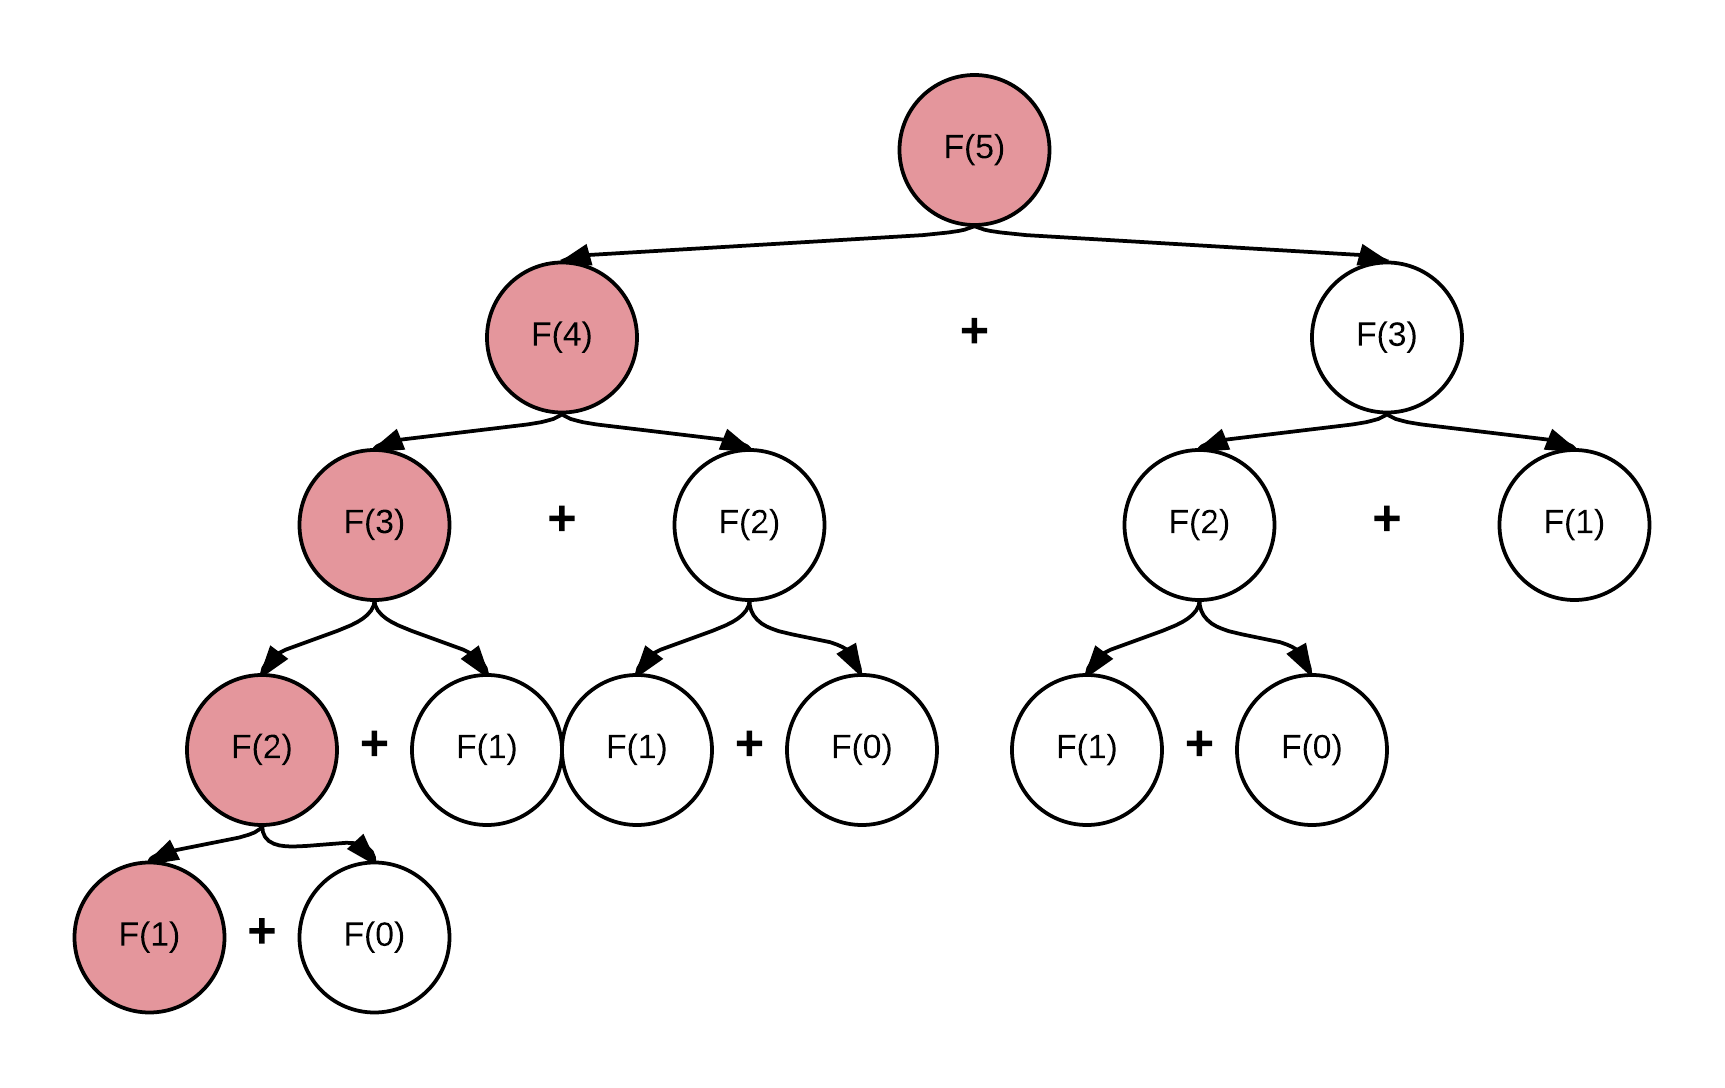
\includegraphics[scale=1]{imagenes/7}
	\caption{Calculos hechos en serie de fibonacci siguiendo perspectiva top-down.}
	\label{fibonacci}
\end{figure}


\begin{conclusion}

A partir de lo ya dicho en la secci�n de ``Validaci�n'', se logr� formular un algoritmo capaz de mejorar la anterior automatizaci�n del recuento de UD's reduciendo considerablemente los tiempos de gran parte de los planes y evidenciar de buena manera el comportamiento que sigue para proximas evaluaciones de los metodos e implementaciones realizadas.

Si bien se encontr� un caso en que el comportamiento no es el �ptimo, se logr� esclarecer las razones constatando c�mo una decisi�n administrativa que afecta la disposici�n de los ramos puede llegar a influir tanto a la descripci�n del avance curricular del alumno como perjudicar el calculo automatizado. 

Como opini�n, se considera que los cambios de la carrera de Ingenier�a Civil Industrial poseen innovaciones en las metodologias o adecuaci�n a las necesidades de los estudiantes, por lo tanto, son medidas atractivas que logran instaurarse dentro del normal desarrollo. Aun as�, debe existir un equilibrio y concenso a nivel de universidad de la instauraci�n de este tipo de medidas en el sentido de que actualmente, como se poseen dominios separados entre departamentos y escuela, se debe velar por el normal funcionamiento local pero a su vez debe existir una cohesi�n para el trabajo en conjunto. Esto incluso implica el asesoramiento que deben tener ciertas implementaciones de normas y reglamentos debido a la falta de visi�n en la posibilidad de implementaci�n que pueden llegar a poseer. Se debe tener cierta certeza de la posibilidad de puesta en marcha antes de firmar un decreto.

Por otra parte, evaluando superficialmente el recuento de UD's en versiones antiguas (por ejemplo en el plan ``Ingenier�a Civil Electricista v2'') se logr� notar ciertos planes que no segu�an un comportamiento logico m�s que el rellenar de alguna manera recuentos que no cumplian todas las reglas (como es el caso de los planes ``Libres''). Esto tambien se debe a que antiguamente el actor principal del proceso tenia la potestad y mayor flexibilidad a la hora de decidir los alumnos con viabilidad de titularse. En cambio, este al ser un sistema automatizado posee mayor rigidez y, si bien en un inicio se poseen planes bien modelados, finalmente se incurre a ``ensuciar'' los planes de estudios a trav�s del tiempo. 

Un ejemplo de esto fue la inclusi�n, hace un tiempo atras, de dos ramos de computaci�n reemplazando el antiguo curso de programaci�n que si bien fue una excelente medida, el modelamiento inicial en el recuento de UD's fue cuestionable y dadas converzaciones termin� ensuciando despreciablemente el plan. Aun as�, recuperando uno de los parrafos mencionados en el ``Marco Te�rico'' acerca de la componente gigante que puede formarse en grafos aleatorios al ir agregando cada vez mas elementos, si bien no es del todo el caso, el ``ensuciar'' de a poco la carrera puede provocar finalmente la generaci�n de una gran componente gigante implicando que parte de las mejoras provocadas en esta memoria debido a la separaci�n de componentes conexas se vea neutralizada.

Por lo anterior, ser�a util la formaci�n de herramientas que permitan guiar y asesorar los lineamientos de los planes de estudios para que si bien permitan innovaciones dentro de �l o la adici�n de elementos creativos, tambien se posea una mirada tecnol�gica con experiencia fundada de la evaluaci�n de dichos planes y vayan analizando a trav�s del tiempo su comportamiento.

\textbf{No se si darle un parrafo a la generalizaci�n que puede darse al recuento en otras facultades como medicina. Generalizar validacion para medi y ver si alcanza el tiempo para agregarlo.}

\end{conclusion}


% \input{glosario.tex} % opcional

\bibliographystyle{plain}
\bibliography{bibliografia}

% \input{anexo_apendices.tex} % opcionales

\end{document}
